\chapter{Determining the presence of NLOS component}

The first set of practical measurements was carried out in order to determine the presence and observe the characteristics of the non-line-of-sight component of the signal. 

\section{Measurements setup}

The measurements were obtained using Nokia's sensing proof-of-concept described in section \ref{sec:intro-PoCarchitecture}. The system was mounted in an indoor scenario, with the receiver positioned at a height of $5,12$ m. The transmitter was positioned towards an open indoor area, located approximately 23 metres away from a warehouse rack (which was in front of a wall) and a cargo door.
The objective was to obtain a non-line-of-sight measurement by reflecting the signal on the wall and subsequently on a moving target. 

The tests were carried out using:

\begin{enumerate}
	\item A human target.
	\item A strong reflector (large metal cabinet with flat surfaces).
\end{enumerate}

The direction (azimuth $\theta$ and elevation $\varphi$) of the transmitted beam was fixed for the whole measurement.

Before each test, a short calibration measure is performed, which includes only the static elements of the scenario. The calibration data will be used in the post-processing steps for subspace-based clutter removal with the CRAP method  \cite{Henninger_Mandelli_Grudnitsky_Wild_Brink_2023}. 

\section{Moving target without obstructions}

The OFDM radar system will be able to determine the range and radial speed component (the angle of arrival AOA is fixed). During the initial measurement the antenna boresight was directed perpendicular to the wall,while the target moved radially between the transmitter and reflector.

Beam elevation was chosen to be as high as possible in order to avoid line-of-sight from the transmitted beam's main lobe. Beam parameters are shown in table \ref{table:Test1TXBeamParams}.


% TODO: substitute placeholder table
\begin{table}[H]
	%\caption*{\textbf{Title of Table (optional)}}
	\centering 
	\begin{tabular}{|p{9em} c c c |}
		\hline
		\rowcolor{bluepoli!40} % comment this line to remove the color
		\textbf{Substitute placeholder table} & \textbf{} & \textbf{} & \textbf{Time aperture [ms]} \T\B \\
		\hline \hline
		$\textbf{Standard frame}$ & 60,91 & 1120 & 10 \T\B \\
		$\textbf{Decimated frame}$ & 45,16 & 24 & 10 \T\B\\
		$\textbf{6 frames}$ & 52,35 & 96 & 60  \T\B\\
		$\textbf{10 frames}$ & 54,66 & 160 & 100  \T\B\\
		
		\hline
	\end{tabular}
	\\[10pt]
	\caption{Transmitted beam parameters for initial measurements.}
	\label{table:Test1TXBeamParams}
\end{table}

Since only the radial component of speed can be measured, the aim of the test was to maximize this component in order to analyze the characteristics of the signal generated from the reflection.

\subsection{Line-of-sight and non-line-of-sight separation}

In addition to clutter removal, calibration measurements provide valuable information for the determination of the distance threshold at which targets can be accurately classified as NLOS. Certain calibration frames can be processed as radar frames, with a focus on analyzing the zero-Doppler component.
	

\begin{figure}[H]
	\centering
	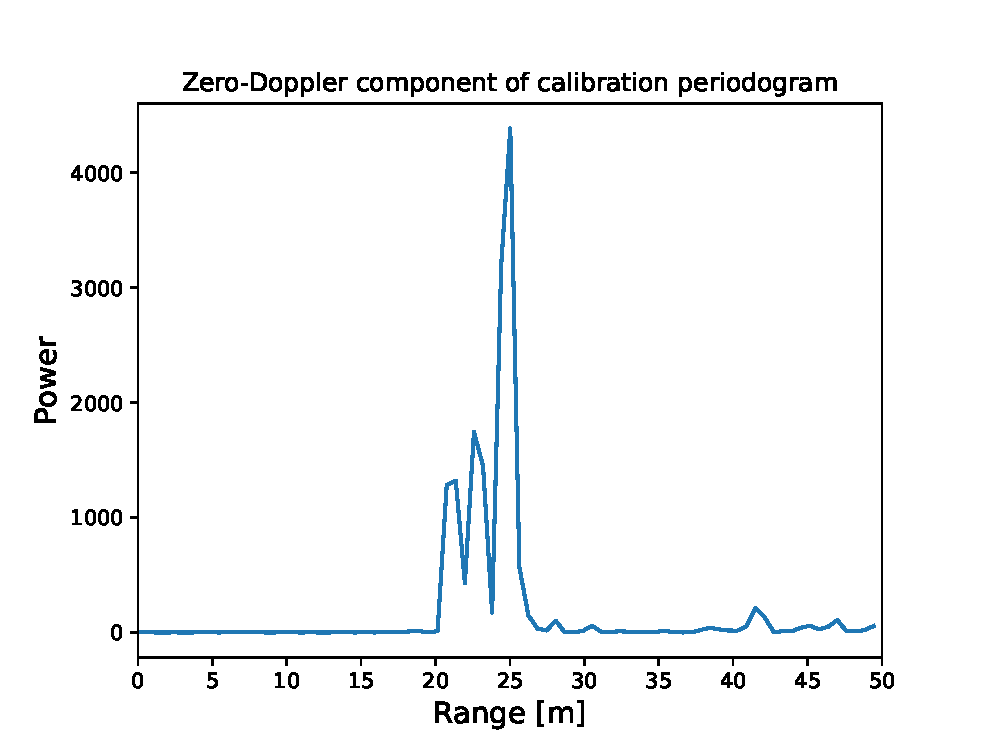
\includegraphics[width=0.6\textwidth]{Images/Test1/cali_static_per_t1.eps}
	\caption{Zero Doppler component of a periodogram generated from calibration measurements.}
	\label{fig:Test1_cali_static_per}
\end{figure}

As can be seen in the figure \ref{fig:Test1_cali_static_per}, a large target is present approximately $23$ m from the system. It was assumed that any target return associated with a range greater than $23$ m was generated by a signal reflected from the main target. The figure also indicates that static clutter has a larger amplitude for ranges greater than $23$ m compared to lower ranges. This is due to the part of the beam that is reflected from the wall towards the environment.
Identifying static NLOS targets from the background was challenging due to the high power of clutter components in the NLOS region, even after clutter removal. However, it was easier to detect obscured targets by analyzing the moving target region of the periodogram. The separation of the regions is highlighted in figure \ref{fig:Test1_nlos_los_separation}.

\begin{figure}[H]
	\centering
	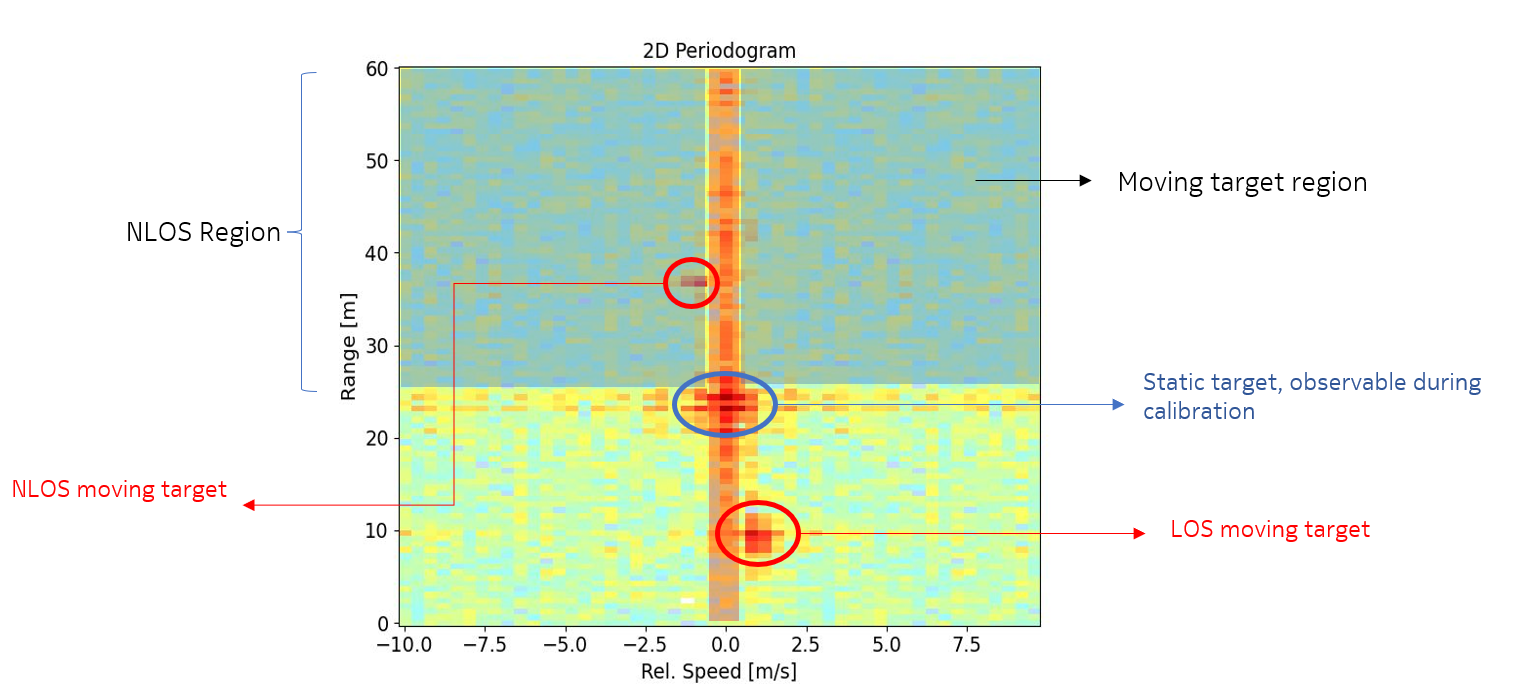
\includegraphics[width=0.9\textwidth]{Images/Test1/nlos-los-separation.png}
	\caption{Processed periodogram, separated in processing regions.}
	\label{fig:Test1_nlos_los_separation}
\end{figure}


After the periodogram has been generated, this separation can be taken into account in the post-processing phase to process the NLOS section separately from the LOS one.

\subsection{Line-of-sight component as ground truth}

Due to the rather large beamwidth of the system, $\pm$7\textdegree\hspace{1pt} in azimuth and elevation, and its sidelobes, the measurement observed the presence of a LOS target return in addition to the expected NLOS one generated by reflection.

During the measurement, the direct component was always visible as no other obstacle was positioned in the scene. It was then decided to use this component and the knowledge of the target geometry to obtain an estimate of the position and velocity of the NLOS return. This estimate was used to check if any of the detected peaks corresponded to the moving target.

\textit{Detection rate} was defined as the metric used to evaluate the experiment: if the speed and range of the detected NLOS target matched the expected value calculated from the LOS component detection, it was considered positive.
The detection rate was then obtained as the ratio between the number of frames in which the NLOS component was above the threshold and the total number of frames in which the LOS component was detected.

\subsection{Processing of the NLOS region}

After defining the two regions of interest from the periodogram, peak detection is conducted separately. A standard strongest peak search is performed for the LOS region, and accurate range and velocity measurements are obtained after interpolation of the adjacent bins.

\begin{figure}[H]
	\centering
	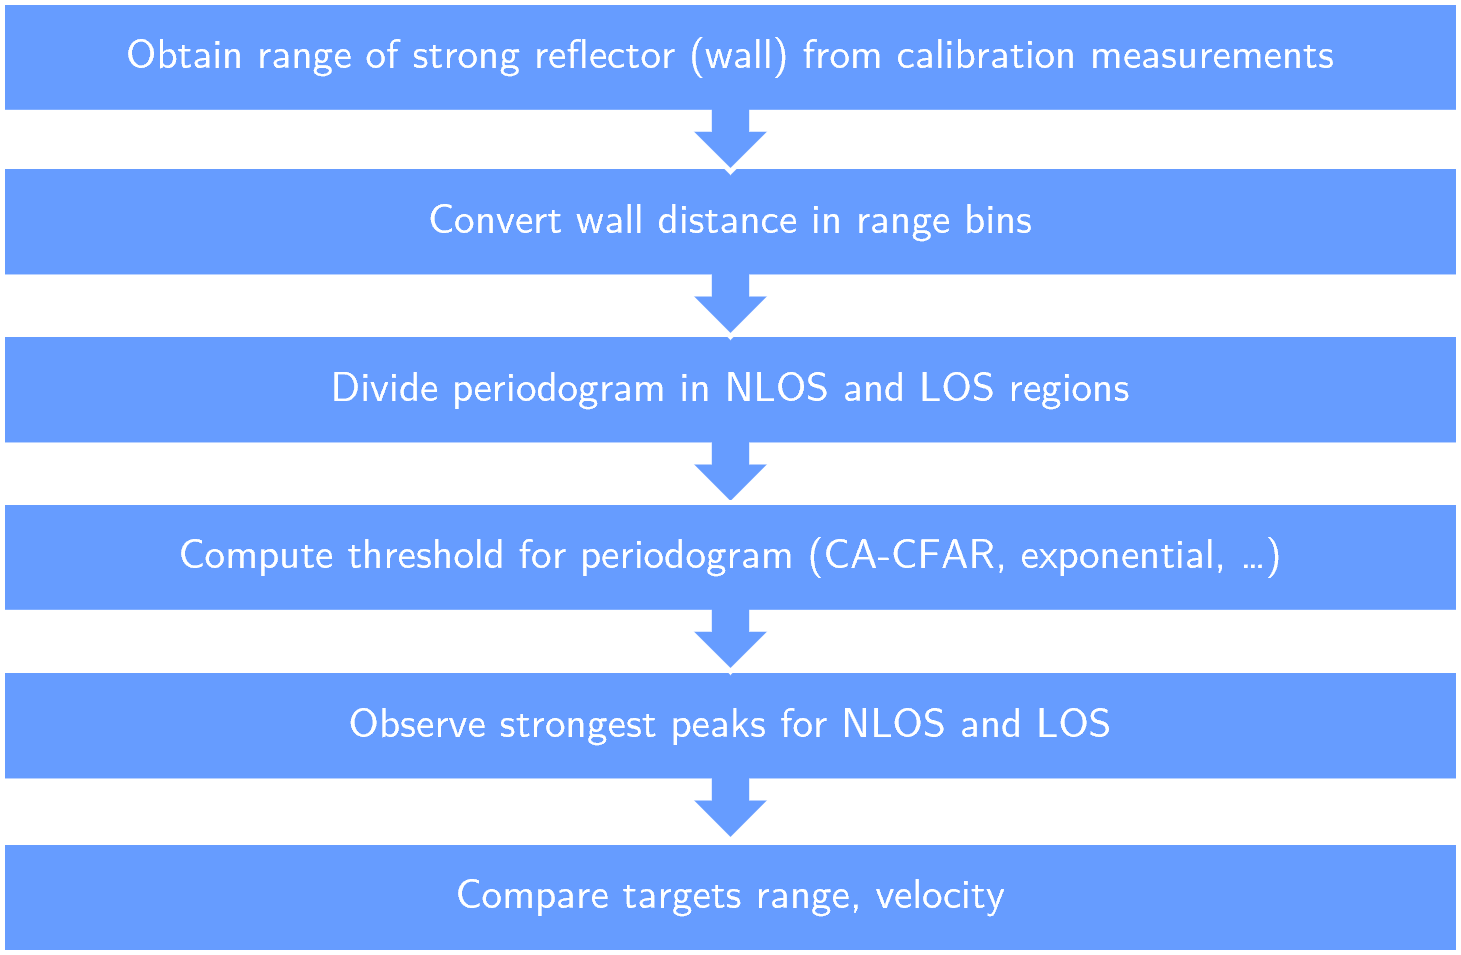
\includegraphics[width=0.9\textwidth]{Images/Test1/NLOS-proc-pipeline.png}
	\caption{Periodogram processing pipeline used for detection tests.}
	\label{fig:Test1_NLOS-proc-pipeline}
\end{figure}


Due to the presence of strong clutter components in the bins close to zero speed, the target search in the NLOS region was performed neglecting this part of the periodogram.

The full process for the experiment is summarized in figure \ref{fig:Test1_NLOS-proc-pipeline}.

